\documentclass[a4paper,11pt]{article}

\usepackage[utf8]{inputenc}

\usepackage{graphicx}
\usepackage{caption}
\usepackage{subcaption}

\usepackage{pgfplots}
\pgfplotsset{compat=1.18} 

\usepackage{minted}
\usepackage{siunitx}

\begin{document}

\title{
    \textbf{Sorting an array in C}
}
\author{Mo Wang}
\date{Spring 2026}

\maketitle

\section*{Introduction}
This report investigates the performance and behavior of different sorting algorithms in C: selection sort, insertion sort, merge sort and quicksort. The primary goal is to analyze and compare their key attributes, including efficiency, time complexity, and practical behavior with a growing size of an array.

Execution time can be measured using the POSIX monotonic clock (\texttt{CLOCK\_MONOTONIC}) which has a granularity of hundreds of nanoseconds. Since each sorting algorithm execution is several orders of magnitudes longer than the clock precision, repeated or batched executions within a single timing measurement is unnecessary for obtaining reliable time measurement. The same algorithm is executed 16 times with randomized arrays, and the minimal time is recorded as it is least affected by operating system scheduling and background process noises.

\subsection*{Selection sort}

Selection sort is a simple iterative sorting algorithm that selects on each iteration the smallest element from the unsorted part of an array, growing from left to right, and swap it with the leftmost element of the unsorted part, right next to the largest element of the sorted part.

\begin{minted}{c}
void selection_sort(int *arr, unsigned int n) {
    if (arr == NULL || n < 2) return;
    for (unsigned int i = 0; i < n - 1; i++) {
        unsigned int min_index = i;
        for (unsigned int j = i + 1; j < n; j++) {
            if (arr[j] < arr[min_index]) {
                min_index = j;
            }
        }
        // swap if a smaller element was found
        if (min_index != i) {
            int temp = arr[i];
            arr[i] = arr[min_index];
            arr[min_index] = temp;
        }
    }
}
\end{minted}

Since the algorithm selects an element from the unsorted part of the array and swaps it with the leftmost element of the unsorted part, it may change the relative order of elements with equal keys, resulting into an unstable algorithm. 

In terms of time complexity, the algorithm performs $n-1$ comparisons on the first iteration between the first element of the array with remaining ones. On the second iteration, the second element is compared with the rest $n-2$ comparisons, and so on. In total, the number of comparisons performed is $\sum_{k=0}^{n-1}{k} = n(n-1)/2 = \frac{n^2}{2}-\frac{n}{2}$. In worst case (a reversed sorted array) up to $n-1$ swaps are performed while in the best case (already sorted array) no swaps occur. Nevertheless, the overall time complexity result into $O(n^2)$ in the best, average, and worst cases.

This quadratic growth is also observable in the measured execution times obtained from benchmarking, as shown in Table~\ref{tab:selection-sort-transposed}

\begin{table}[h]
\begin{center}
\begin{tabular}{l|ccccccc}
\textbf{Size}
    & 1024 & 2048 & 4196 & 8192 & 16384 & 32768 & 65535 \\
\hline
\textbf{ns}
    & $1.1\times10^{6}$
    & $4.6\times10^{6}$
    & $1.9\times10^{7}$
    & $6.9\times10^{7}$
    & $2.8\times10^{8}$
    & $1.2\times10^{9}$
    & $4.6\times10^{9}$ \\
\end{tabular}
\caption{Selection sort: elapsed time per loop (transposed)}
\label{tab:selection-sort-transposed}
\end{center}
\end{table}

In Figure~1, a quadratic equation can be fitted using mathematical regression to model the growth of the measured execution time, which matches closely the measured time.

\begin{figure}[h]
  \centering
  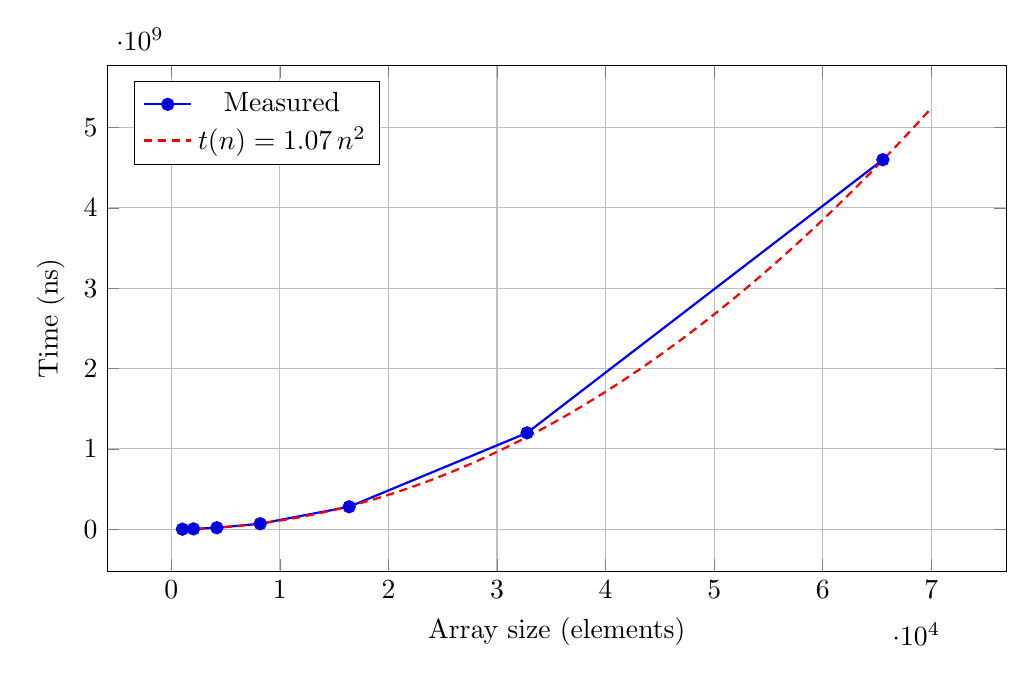
\begin{tikzpicture}
    \begin{axis}[
      xlabel={Array size (elements)},
      ylabel={Time (ns)},
      width=13cm, height=8cm,
      grid=major,
      legend pos=north west,
      ymajorgrids=true,
      xmajorgrids=true
    ]

      % ----------------------------------------------------------
      % Measured data
      % ----------------------------------------------------------
      \addplot+[
        mark=*,
        thick,
        color=blue
      ] coordinates {
        (1024,     1.1e6)
        (2048,     4.6e6)
        (4196,     1.9e7)
        (8192,     6.9e7)
        (16384,    2.8e8)
        (32768,    1.2e9)
        (65535,    4.6e9)
      };
      \addlegendentry{Measured}

      % ----------------------------------------------------------
      % Quadratic fit: t(n) = 1.07 n^2
      % ----------------------------------------------------------
      \addplot[
        red,
        thick,
        densely dashed,
        domain=1000:70000,
        samples=40
      ] {1.07 * x^2};
      \addlegendentry{$t(n)=1.07\,n^{2}$}

    \end{axis}
  \end{tikzpicture}
  \caption{Selection sort benchmark with quadratic regression}
  \label{fig:selection-sort}
\end{figure}

\subsection*{Insertion sort}

Insertion sort is another simple iterative algorithm with slightly better performance than selection sort. Instead of selecting the minimum element of the unsorted part of the array, the algorithm maintain a growing sorted part of the array and inserts the leftmost element of the unsorted part into its expected position within the sorted part by shifting one element at a time. After each iteration, the sorted part of the array grows by one element, from the left up to the current index.

\begin{minted}{c}
void insertion_sort(int *arr, unsigned int n){
    if (arr == NULL || n == 0) return;
    for (unsigned int i = 1; i < n; i++) {
        int hole_element = arr[i];
        unsigned int j = i;
        while (j > 0 && arr[j-1] > hole_element) {
            arr[j] = arr[j-1];
            j--;
        }
        arr[j] = hole_element;
    }
}
\end{minted}

As the sorting algorithm alters the array by shifting one element at a time, the relative order of elements with equal keys will not be disrupted. Hence, insertion sort is a stable algorithm.

\begin{table}[h]
\begin{center}
\begin{tabular}{l|ccccccc}
\textbf{Size}
    & 1024 & 2048 & 4196 & 8192 & 16384 & 32768 & 65535 \\
\hline
\textbf{ns}
    & $6.9\times10^{5}$
    & $2.3\times10^{6}$
    & $9.3\times10^{6}$
    & $3.7\times10^{7}$
    & $1.5\times10^{8}$
    & $5.9\times10^{8}$
    & $2.4\times10^{9}$ \\
\end{tabular}
\caption{Insertion sort: elapsed time per loop (transposed)}
\label{tab:insertion-sort-transposed}
\end{center}
\end{table}

In terms of time complexity, it still remains $O(n^2)$ in worst case (a reversed sorted array), where each incoming element is shifted to the beginning of the array during each iteration. On first iteration (on index 1), only one shift is performed maximal, while in the last iteration where the maximum number of shifts are $n-1$. In this case, the number of shifts are $n(n-1)/2$, resulting into $O(n^2)$ complexity. On the other hand, in the best case (a sorted array), no shift is performed on each iteration, resulting in $O(n)$ time complexity. On average, approximately half of the maximum number of shifts are required, which still leads to an average-case time complexity of $O(n^2)$. However, compared to selection sort, the performance can improve to near-linear complexity if the array is nearly sorted. The execution times shown in Table~\ref{tab:insertion-sort-transposed} are visualized in Figure~2, where a quadratic regression curve closely matches the empirical results.

\begin{figure}[h]
  \centering
  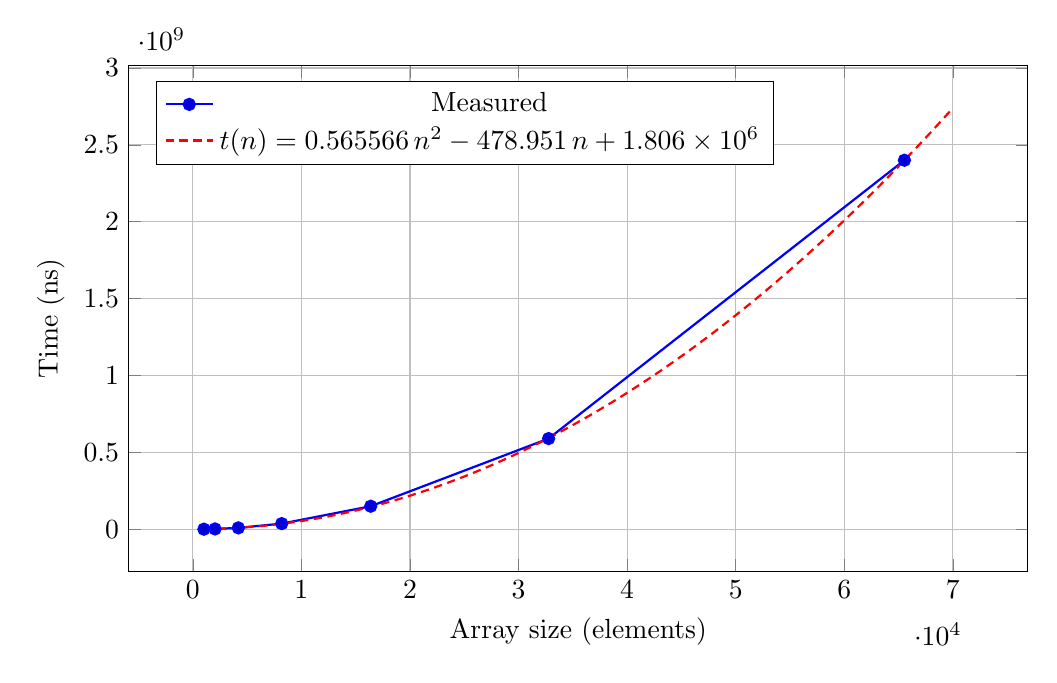
\begin{tikzpicture}
    \begin{axis}[
      xlabel={Array size (elements)},
      ylabel={Time (ns)},
      width=13cm, height=8cm,
      grid=major,
      legend pos=north west,
      ymajorgrids=true,
      xmajorgrids=true
    ]

      % ----------------------------------------------------------
      % Measured Data
      % ----------------------------------------------------------
      \addplot+[
        mark=*,
        thick,
        color=blue
      ] coordinates {
        (1024,     6.9e5)
        (2048,     2.3e6)
        (4196,     9.3e6)
        (8192,     3.7e7)
        (16384,    1.5e8)
        (32768,    5.9e8)
        (65535,    2.4e9)
      };
      \addlegendentry{Measured}

      % ----------------------------------------------------------
      % Quadratic regression: t(n) = a*n^2 + b*n + c
      % a = 0.5655664452, b = -478.9505335, c = 1.805852688e6
      % ----------------------------------------------------------
      \addplot[
        red,
        thick,
        densely dashed,
        domain=1000:70000,   % restrict to data range for speed
        samples=60           % smooth enough, avoids timeout
      ] {0.5655664452*x^2 - 478.9505335*x + 1.805852688e6};
      \addlegendentry{$t(n)=0.565566\,n^{2} - 478.951\,n + 1.806\times10^{6}$}

    \end{axis}
  \end{tikzpicture}
  \caption{Insertion sort benchmark with least-squares quadratic regression}
  \label{fig:insertion-sort}
\end{figure}


\subsection*{Merge sort}

Merge sort, on the other hand, is a recursive sorting algorithm which conceptually split the array into two almost equal parts, with the right one containing at most one element more than left. Afterwards, the left and right subarray, located as two intervals between \texttt{lo} (short for low index) to \texttt{hi} (short for high index), are copied from original array \texttt{org} to another auxillary array \texttt{aux}. Each subarray is sorted recursively and merged afterward together using an efficient linear algorithm (\texttt{merge}). 

The left subarray spans from index \texttt{lo} to the inclusive index \texttt{mid} (middle), while the right subarray spans from index \texttt{mid + 1} to \texttt{hi}.

\begin{minted}{c}
void sort(int * org, int * aux, unsigned int lo, unsigned int hi) {
    if (lo < hi) {
        unsigned int mid = lo + (hi - lo) / 2;
        sort(org, aux, lo, mid);
        sort(org, aux, mid + 1, hi);
        copy_array(org, aux, lo, hi + 1);
        merge(org, aux, lo, mid, hi);
    }
}

\end{minted}

The merge operations combines two sorted subarrays by repeatedly copying the smallest element pointed to by the current indices of each subarray into the original array, until all elements have been merged. The values are read from the auxiliary array \texttt{aux} and written back into the destination array \texttt{org}.

\begin{minted}{c}
void merge(int * org, int * aux, unsigned int lo, unsigned int mid, unsigned int hi) {
    unsigned int i = lo;
    unsigned int j = mid + 1;
    for (unsigned int k = lo; k <= hi; k++) {
        if (i > mid)
            org[k] = aux[j++];
        else if (j > hi)
            org[k] = aux[i++];
        else if (aux[i] <= aux[j])
            org[k] = aux[i++];
        else
            org[k] = aux[j++];
    }
}
\end{minted}

From a stability perspective, mergesort is a stable algorithm. During the each merge step, the only step where reordering occurs, the element from the left subarray is selected first when two elements from respective array are same. Since the left subarray contains elements that originally appeared earlier in the input array, their relative order is preserved.

Since the array is recursively divided into smaller subarrays, the recursion continues until subarrays of size one are reached. As the array is approximately halved at each recursive call, the total number of recursive levels is $\left \lceil{log_2(n)}\right \rceil $. At each recursive depth, the merge step processes all elements exactly once. That means on total, $n$ elements are copied from multiple subarray intervals in original array to auxiliary array, while $n$ elements are compared and copied back to original array during array merge. Therefore, the total amount of work performed at each recursive level is linear $O(n)$. In total, repeating linear-time work with logarithmic-time recursive depth yields time complexity $O(n\cdot log(n))$, which can be visualized using a fitted regression equation in Figure 3 with measurement data in Table 3.

\begin{table}[h]
\begin{center}
\begin{tabular}{l|ccccccc}
\textbf{Size}
    & 1024 & 2048 & 4196 & 8192 & 16384 & 32768 & 65535 \\
\hline
\textbf{ns}
    & $1.1\times10^{5}$
    & $2.3\times10^{5}$
    & $4.5\times10^{5}$
    & $9.1\times10^{5}$
    & $2.0\times10^{6}$
    & $4.3\times10^{6}$
    & $9.4\times10^{6}$ \\
\end{tabular}
\caption{Merge sort: elapsed time per loop (transposed)}
\label{tab:mergesort-transposed}
\end{center}
\end{table}

\begin{figure}[h]
  \centering
  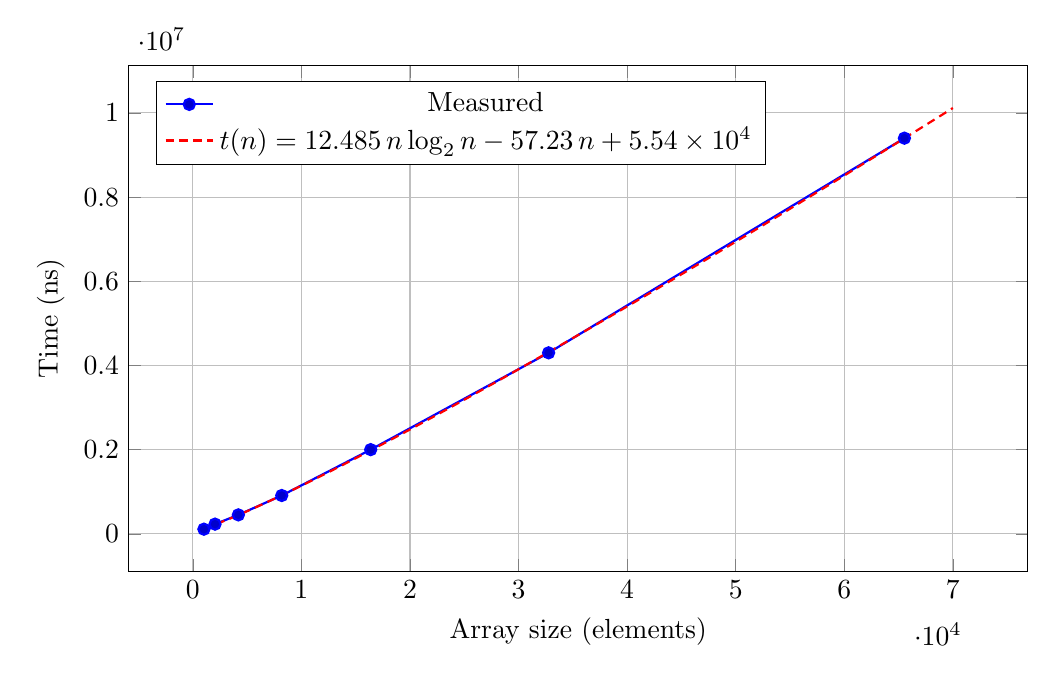
\begin{tikzpicture}
    \begin{axis}[
      xlabel={Array size (elements)},
      ylabel={Time (ns)},
      width=13cm, height=8cm,
      grid=major,
      legend pos=north west,
      ymajorgrids=true,
      xmajorgrids=true
    ]

      % ----------------------------------------------------------
      % Measured data
      % ----------------------------------------------------------
      \addplot+[
        mark=*,
        thick,
        color=blue
      ] coordinates {
        (1024,     1.1e5)
        (2048,     2.3e5)
        (4196,     4.5e5)
        (8192,     9.1e5)
        (16384,    2.0e6)
        (32768,    4.3e6)
        (65535,    9.4e6)
      };
      \addlegendentry{Measured}

      % ----------------------------------------------------------
      % Improved regression:
      % t(n) = a*n*log2(n) + b*n + c
      % a = 12.4848689709, b = -57.2304548517, c = 55401.3997885
      % ----------------------------------------------------------
      \addplot[
        red,
        thick,
        densely dashed,
        domain=1000:70000,   % restrict to data range for speed
        samples=60
      ]
      {12.4848689709 * x * (ln(x)/ln(2)) + (-57.2304548517) * x + 55401.3997885};
      \addlegendentry{$t(n)=12.485\,n\log_{2}n - 57.23\,n + 5.54\times10^{4}$}

    \end{axis}
  \end{tikzpicture}
  \caption{Merge sort benchmark with improved $n\log n$ regression (tail-aligned)}
  \label{fig:mergesort}
\end{figure}

\subsection*{Improved merge sort}

The merge sort algorithm can also be further improved the roles of the auxiliary array and the original array in each recursive call, in order to avoid copying the full array. Instead of copying the current subarray from \texttt{org} to \texttt{aux} at every level, the source and destination array roles are exchanged, while maintaining same merge logic. This is because that each recursive call only operates on a narrowed subarray range, which does not affect the elements outside the range.

As the improved version doesn't involves changes in merge step, where array reordering occurs, the algorithm is still stable.

\begin{minted}{c}
void sort(int * org, int * aux, unsigned int lo, unsigned int hi) {
    if (lo < hi) {
        unsigned int mid = lo + (hi - lo) / 2;
        sort(aux, org, lo, mid);
        sort(aux, org, mid + 1, hi);
        merge(org, aux, lo, mid, hi);
    }
}
\end{minted}

Similar to merge sort, the time complexity remains $O(n\cdot\log(n))$, which can be conformed by the fitted equation from regression in Figure 4, to the measured execution time in Table 4.

\begin{table}[h]
\begin{center}
\begin{tabular}{l|ccccccc}
\textbf{Size}
    & 1024 & 2048 & 4196 & 8192 & 16384 & 32768 & 65535 \\
\hline
\textbf{ns}
    & $9.4\times10^{4}$
    & $1.9\times10^{5}$
    & $3.8\times10^{5}$
    & $7.2\times10^{5}$
    & $1.6\times10^{6}$
    & $3.4\times10^{6}$
    & $7.8\times10^{6}$ \\
\end{tabular}
\caption{Simple merge sort: elapsed time per loop (transposed)}
\label{tab:simple-mergesort-transposed}
\end{center}
\end{table}

\begin{figure}[h]
  \centering
  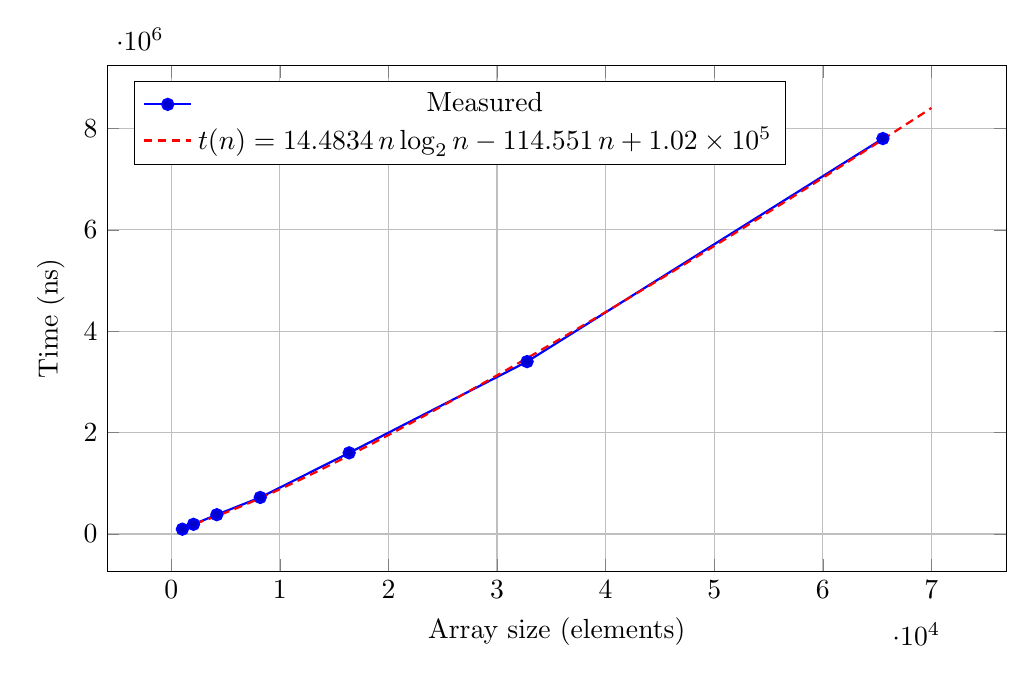
\begin{tikzpicture}
    \begin{axis}[
      xlabel={Array size (elements)},
      ylabel={Time (ns)},
      width=13cm, height=8cm,
      grid=major,
      legend pos=north west,
      ymajorgrids=true,
      xmajorgrids=true
    ]

      % ----------------------------------------------------------
      % Measured data
      % ----------------------------------------------------------
      \addplot+[
        mark=*,
        thick,
        color=blue
      ] coordinates {
        (1024,     9.4e4)
        (2048,     1.9e5)
        (4196,     3.8e5)
        (8192,     7.2e5)
        (16384,    1.6e6)
        (32768,    3.4e6)
        (65535,    7.8e6)
      };
      \addlegendentry{Measured}

      % ----------------------------------------------------------
      % Improved regression:
      % t(n) = a*n*log2(n) + b*n + c
      % a = 14.4834478744, b = -114.551055308, c = 1.02324e5
      % ----------------------------------------------------------
      \addplot[
        red,
        thick,
        densely dashed,
        domain=1000:70000,   % restrict to data range for speed
        samples=60
      ]
      {14.4834478744 * x * (ln(x)/ln(2)) + (-114.551055308) * x + 1.02324e5};
      \addlegendentry{$t(n)=14.4834\,n\log_{2}n - 114.551\,n + 1.02\times10^{5}$}

    \end{axis}
  \end{tikzpicture}
  \caption{Simple merge sort benchmark with improved $n\log n$ regression (tail-aligned)}
  \label{fig:simple-mergesort}
\end{figure}

\subsection*{Quick sort}

Quick sort is a recursive sorting algorithm that selects a pivot element as the middlemost element in the array and partitions the remaining elements into two subarrays: one containing elements larger than the pivot element and the other smaller than pivot. Each subarray is then recursively sorted, until subarrays of size one is reached. Finally, the subarrays are combined to produce the fully sorted array.

During the partitioning step, elements are swapped only based on comparisons with the pivot element. As a result, the relative order of elements with equal keys is not preserved, making quick sort an unstable sorting algorithm.

Partitioning is performed using two index pointers starting from opposite ends of the subarray and moving toward each other. Whenever an element on the left pointer is larger than the pivot and an element on the right pointer is smaller, the two elements are swapped. This process continues until the pointers are met in pivot element, whereas a boundary between i and j index is drawn. The elements left to the boundary are less or equals to pivot element while the elements on the right side are larger than pivot.

\begin{minted}{c}
void quick_sort(int *arr, unsigned start, unsigned int end){
    if (start >= end) return;
    if (end - start <= 1) return;
    unsigned int pivot_index = (start + end)/2;
    int pivot_value = arr[pivot_index];
    unsigned int i = start;
    unsigned int j = end - 1;
    while (i < j){
        while (arr[i] < pivot_value && i < end) i++;
        while (arr[j] > pivot_value && j > start) j--;
        if (i < j){
            int temp = arr[i];
            arr[i] = arr[j];
            arr[j] = temp;
            i++;
            j--;
        }
    }

    quick_sort(arr, start, i);
    quick_sort(arr, i, end);
}
\end{minted}

Similar to merge sort, the array is recursively divided into two smaller subarrays on each recursive call until subarrays of size one are reached. Each division does not guarantee equally divided subarrays on each partition, resulting in $n-1$ call depth in the worst case (selected pivot is smallest or largest element of the array). In the best case, the pivot is median value of the array, resulting in perfectly divided sub-arrays and $\log_2(n)$ call depth. Additionally, in each recursive depth, the partitioning step processes all elements of the array at most exactly once, meaning $n$ elements are compared and swapped, resulting in linear growth. In total, in the best case, the time complexity results in $O(n\cdot\log(n))$ with $log_2(n)$ call depth with each processing $n$ elements. However, in the worst case the time complexity can degrade to $O(n^2)$ time complexity, as call depth reaches $n$. In average case, the partition step can be modeled as dividing the array into two subarrays of expected sizes $\frac{n}{4}$ and ${\frac{3n}{4}}$. Time recurrence relation can be described as $t(n)=t(\frac{n}{4}) + t(\frac{3n}{4}) + cn$, whereas $cn$ is partitioning work. The recursion depth is determined by the larger subproblem, which decreases geometrically as $n{\frac{3}{4}}^k$ on depth $k$. As it approaches 1, the largest number of recursive depth is logarithmic, by solving $n(\frac{3}{4})^k=1$.

The logarithmic time complexity can be visualized in Figure 5 with a fitted regression equation from the empirical execution time in Table 5.

\begin{table}[h]
\begin{center}
\begin{tabular}{l|ccccccc}
\textbf{Size}
    & 1024 & 2048 & 4196 & 8192 & 16384 & 32768 & 65535 \\
\hline
\textbf{ns}
    & $9.4\times10^{4}$
    & $1.9\times10^{5}$
    & $3.8\times10^{5}$
    & $7.2\times10^{5}$
    & $1.6\times10^{6}$
    & $3.4\times10^{6}$
    & $7.8\times10^{6}$ \\
\end{tabular}
\caption{Simple merge sort: elapsed time per loop (transposed)}
\label{tab:simple-mergesort-transposed}
\end{center}
\end{table}

\begin{figure}[h]
  \centering
  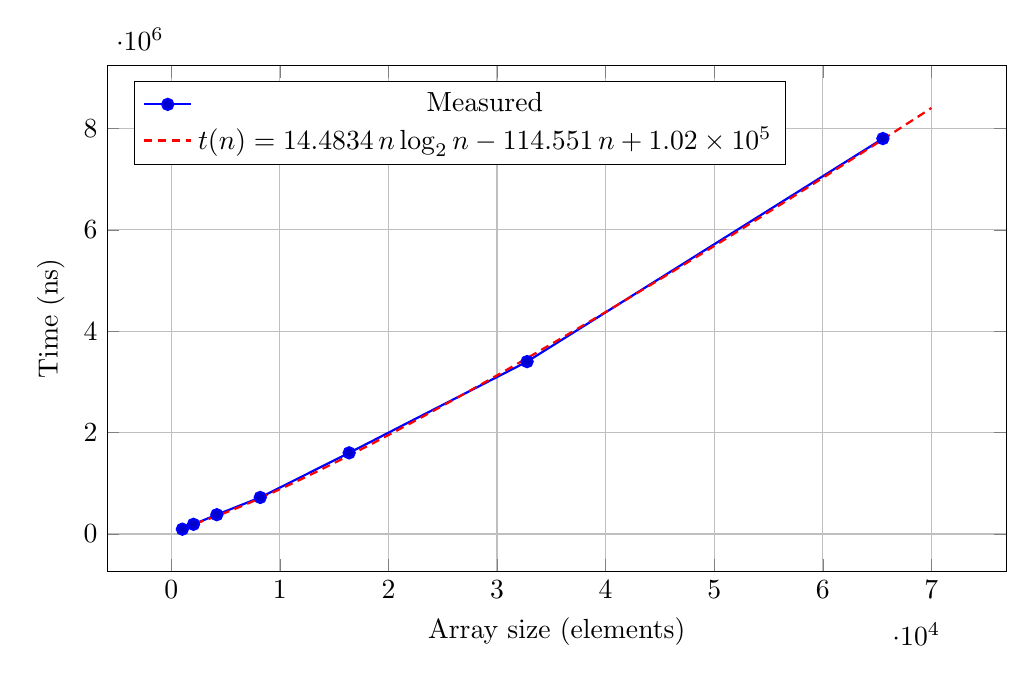
\begin{tikzpicture}
    \begin{axis}[
      xlabel={Array size (elements)},
      ylabel={Time (ns)},
      width=13cm, height=8cm,
      grid=major,
      legend pos=north west,
      ymajorgrids=true,
      xmajorgrids=true
    ]

      % ----------------------------------------------------------
      % Measured data
      % ----------------------------------------------------------
      \addplot+[
        mark=*,
        thick,
        color=blue
      ] coordinates {
        (1024,     9.4e4)
        (2048,     1.9e5)
        (4196,     3.8e5)
        (8192,     7.2e5)
        (16384,    1.6e6)
        (32768,    3.4e6)
        (65535,    7.8e6)
      };
      \addlegendentry{Measured}

      % ----------------------------------------------------------
      % Improved regression:
      % t(n) = a*n*log2(n) + b*n + c
      % a = 14.4834478744, b = -114.551055308, c = 1.02324e5
      % ----------------------------------------------------------
      \addplot[
        red,
        thick,
        densely dashed,
        domain=1000:70000,   % restrict to data range for speed
        samples=60
      ]
      {14.4834478744 * x * (ln(x)/ln(2)) + (-114.551055308) * x + 1.02324e5};
      \addlegendentry{$t(n)=14.4834\,n\log_{2}n - 114.551\,n + 1.02\times10^{5}$}

    \end{axis}
  \end{tikzpicture}
  \caption{Simple merge sort benchmark with improved $n\log n$ regression (tail-aligned)}
  \label{fig:simple-mergesort}
\end{figure}


\section*{Conclusion}

To sum up, both quick sort and merge sort outperform selection sort and insert sort, since the first two sort algorithm have a time complexity $O(n\cdot\log(n))$, while the latter two have a quadratic time complexity $(n^2)$. This theoretical difference is reflected in the empirical benchmark results which are visualized in Figure 6, where merge sort and quick sort scale much more efficiently as the array size increases. Judging the empirical data, mergesort and quicksort are hundreds times faster than selection sort and merge sort.

Between the two quadratic algorithms, insertion sort consistently outperforms selection sort on average, as it terminates early when elements are already close to their intended positions. As a result, the algorithm is well-suited for nearly sorted arrays. In contrast, selection sort performs the same number of comparisons regardless of array element order.

Between the two linear-logarithmic algorithms, performance comparasions cannot be determined, since both are logarithmic. Merge sort, on one hand, introduces a slight performance overhead of allocating and copying elements into an auxiliary array compared to quicksort, while quicksort, on other hand, can degrade to $O(n^2)$ time complexity.

In terms of stability, merge sort and insertion sort preserve the relative order of elements with equal keys, while selection sort and quick sort do not. Additionally, merge sort provides the best balance between performance and stability, whereas quick sort, despite being unstable, remains attractive in practice due to its low constant factors and efficient in-place behavior.

\begin{figure}[h]
  \centering
  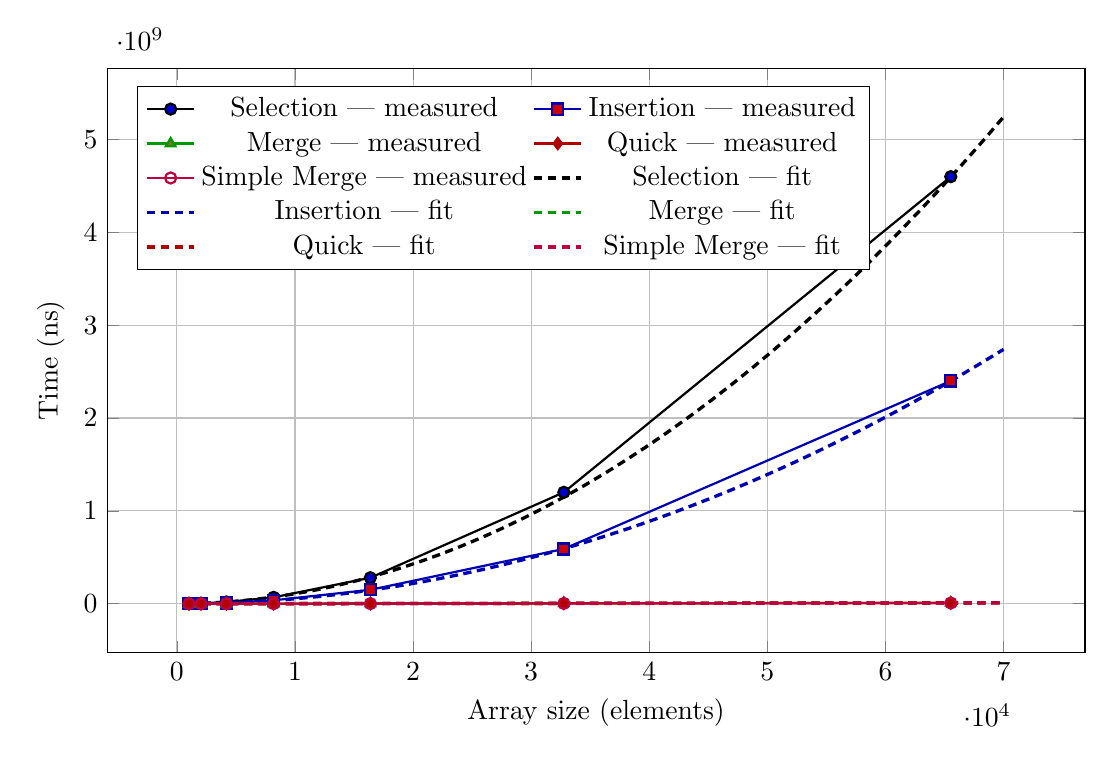
\begin{tikzpicture}
    \begin{axis}[
      xlabel={Array size (elements)},
      ylabel={Time (ns)},
      width=14cm, height=9cm,
      grid=major,
      legend pos=north west,
      legend columns=2,
      ymajorgrids=true,
      xmajorgrids=true,
      % ymode=log,           % ← 如需对数纵轴可取消注释
      % log basis y=10,
    ]

      % =========================== Measured Data ===========================
      % Selection Sort (measured)
      \addplot+[
        mark=*,
        thick,
        color=black
      ] coordinates {
        (1024,     1.1e6)
        (2048,     4.6e6)
        (4196,     1.9e7)
        (8192,     6.9e7)
        (16384,    2.8e8)
        (32768,    1.2e9)
        (65535,    4.6e9)
      };
      \addlegendentry{Selection — measured}

      % Insertion Sort (measured)
      \addplot+[
        mark=square*,
        thick,
        color=blue!70!black
      ] coordinates {
        (1024,     6.9e5)
        (2048,     2.3e6)
        (4196,     9.3e6)
        (8192,     3.7e7)
        (16384,    1.5e8)
        (32768,    5.9e8)
        (65535,    2.4e9)
      };
      \addlegendentry{Insertion — measured}

      % Merge Sort (measured)
      \addplot+[
        mark=triangle*,
        thick,
        color=green!60!black
      ] coordinates {
        (1024,     1.1e5)
        (2048,     2.3e5)
        (4196,     4.5e5)
        (8192,     9.1e5)
        (16384,    2.0e6)
        (32768,    4.3e6)
        (65535,    9.4e6)
      };
      \addlegendentry{Merge — measured}

      % Quick Sort (measured)
      \addplot+[
        mark=diamond*,
        thick,
        color=red!70!black
      ] coordinates {
        (1024,     9.9e4)
        (2048,     2.1e5)
        (4196,     4.3e5)
        (8192,     9.1e5)
        (16384,    1.9e6)
        (32768,    4.3e6)
        (65535,    9.2e6)
      };
      \addlegendentry{Quick — measured}

      % Simple Merge Sort (measured)
      \addplot+[
        mark=o,
        thick,
        color=purple
      ] coordinates {
        (1024,     9.4e4)
        (2048,     1.9e5)
        (4196,     3.8e5)
        (8192,     7.2e5)
        (16384,    1.6e6)
        (32768,    3.4e6)
        (65535,    7.8e6)
      };
      \addlegendentry{Simple Merge — measured}

      % =========================== Fits (Overleaf-safe) ===========================
      % Selection Sort fit: t = 1.07 n^2
      \addplot[
        black, densely dashed, very thick,
        domain=1000:70000, samples=40
      ] {1.07 * x^2};
      \addlegendentry{Selection — fit}

      % Insertion Sort fit: t = 0.565566 n^2 - 478.951 n + 1.806e6
      \addplot[
        blue!70!black, densely dashed, very thick,
        domain=1000:70000, samples=40
      ] {0.5655664452 * x^2 - 478.9505335 * x + 1.805852688e6};
      \addlegendentry{Insertion — fit}

      % Merge Sort fit: t = 12.484869 n log2 n - 57.2305 n + 5.54014e4
      \addplot[
        green!60!black, densely dashed, very thick,
        domain=1000:70000, samples=40
      ] {12.4848689709 * x * (ln(x)/ln(2)) + (-57.2304548517) * x + 55401.3997885};
      \addlegendentry{Merge — fit}

      % Quick Sort fit: t = 11.099638 n log2 n - 37.434 n + 2.49031e4
      \addplot[
        red!70!black, densely dashed, very thick,
        domain=1000:70000, samples=40
      ] {11.0996381095 * x * (ln(x)/ln(2)) + (-37.4339527432) * x + 2.49031e4};
      \addlegendentry{Quick — fit}

      % Simple Merge Sort fit: t = 14.483448 n log2 n - 114.551 n + 1.02324e5
      \addplot[
        purple, densely dashed, very thick,
        domain=1000:70000, samples=40
      ] {14.4834478744 * x * (ln(x)/ln(2)) + (-114.551055308) * x + 1.02324e5};
      \addlegendentry{Simple Merge — fit}

    \end{axis}
  \end{tikzpicture}
  \caption{Comparison of Selection, Insertion, Merge, Quick, and Simple Merge Sort (measured vs. fitted)}
  \label{fig:sorts-comparison-5}
\end{figure}

\end{document}